\documentclass[14pt, fleqn, xcolor={dvipsnames, table}]{beamer}
\usepackage[T2A]{fontenc}
\usepackage[utf8]{inputenc}
\usepackage[english,russian]{babel}
\usepackage{amssymb,amsfonts,amsmath,mathtext}
\usepackage{cite,enumerate,float,indentfirst}
\usepackage{cancel}
\usepackage{graphicx}
\usepackage{animate}

\usepackage{tikz}
% \usepackage{enumitem}
\usetikzlibrary{shadows}

% \usepackage{enumitem}
% \setitemize{label=\usebeamerfont*{itemize item}%
%   \usebeamercolor[fg]{itemize item}
%   \usebeamertemplate{itemize item}}

\graphicspath{{images/}}

\usetheme{Madrid}
\usecolortheme{seahorse}
\renewcommand{\CancelColor}{\color{red}}

\setbeamercolor{footline}{fg=Blue!50}
\setbeamertemplate{footline}{
  \leavevmode%
  \hbox{%
  \begin{beamercolorbox}[wd=.333333\paperwidth,ht=2.25ex,dp=1ex,center]{}%
    И. Кураленок, Н. Поваров, Яндекс
  \end{beamercolorbox}%
  \begin{beamercolorbox}[wd=.333333\paperwidth,ht=2.25ex,dp=1ex,center]{}%
    Санкт-Петербург, 2014
  \end{beamercolorbox}%
  \begin{beamercolorbox}[wd=.333333\paperwidth,ht=2.25ex,dp=1ex,right]{}%
  Стр. \insertframenumber{} из \inserttotalframenumber \hspace*{2ex}
  \end{beamercolorbox}}%
  \vskip0pt%
}
\newcommand\indentdisplays[1]{%
     \everydisplay{\addtolength\displayindent{#1}%
     \addtolength\displaywidth{-#1}}}
\newcommand{\itemi}{\item[\checkmark]}

\newenvironment{mydescription}[1]
  {\begin{list}{}%
   {\renewcommand\makelabel[1]{\color{blue}##1:\hfill}%
   \settowidth\labelwidth{\makelabel{#1}}%
   \setlength\leftmargin{\labelwidth}
   \addtolength\leftmargin{\labelsep}}}
  {\end{list}}

\title{Уменшение размерности: обзор\\\small{}}
\author[]{\small{%
И.~Куралёнок,
Н.~Поваров}}
\date{}
\begin{document}

\begin{frame}
\maketitle
\small
\begin{center}
\vspace{-60pt}
\normalsize {\color{red}Я}ндекс \\
\vspace{80pt}
\footnotesize СПб, 2014
\end{center}
\end{frame}
\section{Чем feature extraction отличается от развешивания датчиков?}

\begin{frame}{Область применения}{Feature extraction}
\textbf{Зачем:} наглядность (быть аккуратными!), экономия ресурсов обучения и использования (предобработка), прибрать шум, гибкость в построении данных. \\
\textbf{Когда:}
\begin{itemize}
  \item несколько факторов про одно, но все глядят в разные стороны из-за особенностей реализации;
  \item хотим структурировать обучение: сначала одну часть подобрать, потом другую, а потом все вместе;
  \item понимаем структуру данных.
\end{itemize}
\end{frame}

\begin{frame}{Feature extraction}
Хотим научиться комбинировать существующие сигналы делая их более доступными для используемого метода обучения.\\
Какие тут есть задачи?
\begin{itemize}
  \item \only<1>{Собрать что-то более удобное}
  \only<2->{\textbf{Собрать что-то более удобное}}
  \item Понять что-то новое о данных (data mining)
\end{itemize}
\end{frame}

\begin{frame}{Как отличить extraction от датчиков?}{Пример с мобильниками}
Как понять каким образом человек передвигается?\\
{\color{blue} Датчики:} повесим специальный датчик \\
{\color{blue} FE:} соберем данные от пользователей и спомощью существующих датчиков предскажем.
\end{frame}

\begin{frame}{Как отличить extraction от датчиков?}{Пример с депутатами}
Приходит к депутатам проситель, им надо принять решение, однако сами они не могут выбрать, так как информация неструктурированна. Структурировать ее можно с помощью анкеты.\\
Анкета, заполненная посетителем --- датчик; \\
Анкета, заполненная помощником (немым) ---  extraction.
\end{frame}

\begin{frame}{Как отличить extraction от датчиков?}{Выводы}
Во многом вопрос философский, однако rule of thumb такой:\\
\textit{Если фактор не несет новой информации о вселенной, он extraction, иначе --- новый фактор.}\\
~\\
C другой стороны все зависит от постановки, например в одной постановке изучаемой вселенной могут быть существующие логи, в другой --- пользователи. В разных парадигмах получим разные результаты. 
\end{frame}

\begin{frame}{Какие есть способы собрать что-то удобное?}
\begin{itemize}
  \item Без использования дополнительных данных (какая-то нормализация)
  \begin{itemize}
    \item с точки зрения линейной алгебры (PCA/Kernel PCA)
    \item с точки зрения разделения сигналов (ICA)
    \item группировка (кластеризация)
    \item какие-то еще принципы, специфичные для данных (например поделить голосовой сигнал)
  \end{itemize}
  \item С дополнительными данными
  \begin{itemize}
    \item Metric learning
    \item Хитрая кластеризация с предпочтениями
    \item Transfer learning
  \end{itemize}
\end{itemize}
\end{frame}

\section{PCA}

\begin{frame}{Метод главных компонент}{Из определения}
{\color{blue}Задача:} превратить множество скоррелированных сигналов в множество линейно некоррелирующих с помощью поворота:
$$\begin{array}{l}
\min \sum_{(i,j)} y_i^T y_j \\
X = Q^T Y Q \\
q_i^T q_j = 0, \forall i \ne j \\
q_i^T q_i = 1, \forall i 
\end{array}$$
Мы знаем хотя бы одно решение такой задачи! При этом не все строки в $Y$ одинаково полезны. Отсортируем их по модулю.
\end{frame}

\begin{frame}{Метод главных компонент}{Альтернативный способ: отсосы}
Попробуем итеративно выбирать направление, несущее наибольшую ``информацию'' (на самом деле дисперсию):
$$\begin{array}{l}
\arg \max_{\|w\|_2=1} \sum_i (x_i^Tw)^2 \\
\arg \max_{\|w\|_2=1} w^T X^TXw \\
\arg \max_{w} {w^T X^TXw \over w^Tw} \\
\end{array}$$
Это Rayleigh Quotient, для которого известно решение -- главный собственный вектор.
\end{frame}

\begin{frame}{Как реализовать PCA?}
\begin{itemize}
  \item Можно искать корни уравнения $det\|X - \lambda E\| = 0$, но мы так делать не будем
  \item Возведение в степень (power iteration)
  \item Оптимизированный способ через пространство Крылова (Lanczos, например)
  \item Последовательное LQ (QR) разложение:
$$
A_{k+1} = R_k Q_k = Q_k^TQ_kR_kQ_k=Q_k^TA_kQ_k
$$
\end{itemize}
\end{frame}

\begin{frame}{Свойства PCA}
\begin{itemize}
  \item Все хорошо, когда пространство похоже на нормальное распределение. Однако на практике это обычно не так:
  \only<2>{\begin{center}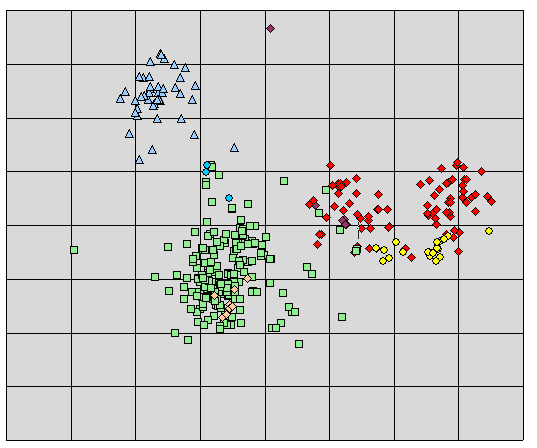
\includegraphics[width=0.6\textwidth]{pca.png}\end{center}}
  \only<3->{\item Мы рассмотрели линейную зависимость, а что если она нелинейна?}
\end{itemize}
\uncover<4->{$\Rightarrow$ попробуем стандартный фокус с kernel}
\end{frame}

\section{Kernel PCA}
\begin{frame}{Kernel PCA}
\footnotesize
Хотим решить задачу PCA в каком-то другом пространстве, образованном из данного через преобразование $\Phi$. Для этого нам нужно лишь узнать проекции на собственные вектора $\Phi(x)^T v_k$. Для этого воспользуемся таким:
$$\begin{array}{l}
\lambda v = Cv \\
x^T v = \frac{1}{\lambda} x^T Cv \\
v = \sum a_i \Phi(x_i)
\end{array}$$
Все это добро выполняется для точек из $X$. Представим, что kernel space имеет размерность $N$.
$$
N \lambda K a = K^2 a
$$
Решив это уравнение, получим разложение любого $\Phi(x)$ по $V$
$$
\Phi(x)^Tv_k = \frac{1}{\lambda_k} \sum_i a_i K(x, x_i)
$$
\end{frame}

\section{ICA}
\begin{frame}{Общая схема ICA}
Представим сигнал как сумму независимых например так:
$$y = w^T \mathcal{N}(0, \Sigma) + \mathcal{N}(0,\delta)$$
\only<1>{Теперь наша задача подобрать такие $(w, \Sigma, \delta)$, которые будут наилучшим образом объяснять данные.}
\only<2->{Теперь наша задача подобрать такие $(w, \Sigma, \delta)$, которые будут \textit{наилучшим образом} \textit{объяснять} данные.}
\uncover<3>{Это можно делать по тем же принципам что и PCA:
\begin{itemize}
  \item получше объяснить данные (ICA on LL/Infomax/KL/etc.);
  \item выделяя самые ``жирные'' направления по-одному (Projection Pursuit)
\end{itemize}}
\end{frame}

\begin{frame}{Реализация ICA}
Сильно зависит от конкретной задачи. 
\end{frame}

\subsection{Через variational bayes}

\subsection{Через ``ненормальность''}
\end{document}
